\documentclass{article}[12pt]
\renewcommand{\baselinestretch}{1.5}

\usepackage[affil-it]{authblk}
\usepackage[space]{grffile}

\usepackage[a4paper]{geometry}
\geometry{verbose}
\usepackage{float}
\usepackage{graphicx}
\usepackage{setspace}
\usepackage{caption}

\usepackage[utf8]{inputenc}
\usepackage[english]{babel}

\usepackage{latexsym,textcomp,longtable,tabulary}
\usepackage{booktabs,array,multirow}
\usepackage{amsfonts,amsmath,amssymb,mathbbol,calc}
\usepackage{subfigure,color,blindtext,enumitem,siunitx}

\usepackage{mathtools}
\usepackage{url,hyperref,etoolbox}
\numberwithin{equation}{section}
\hypersetup{colorlinks=false,pdfborder={0 0 0}}

%+figure layout options
\restylefloat{figure}
\setlist{leftmargin=*,before=\setlength{\rightmargin}{\leftmargin}}
%-figure layout options

\providecommand\citet{\cite}
\providecommand\citep{\cite}
\providecommand\citealt{\cite}


\makeatletter
\makeatother


\newif\iflatexml\latexmlfalse
\providecommand{\tightlist}{\setlength{\itemsep}{0pt}\setlength{\parskip}{0pt}}%
\AtBeginDocument{\DeclareGraphicsExtensions{.pdf,.PDF,.eps,.EPS,.png,.PNG,.tif,.TIF,.jpg,.JPG,.jpeg,.JPEG}}
\begin{document}

\title{
On the affect of the Laplacian in equlibration
dynamics of the Spherical Model
}

\author{Gregory Szep}
\affil{King's College London}
\date{\today}

\maketitle
Consider a system of $N$ linearly interacting degrees of freedom. We collect
them into a vector $\bar{\mathbf{s}}(t) = \left(\,s_1(t),\cdots, s_N(t)\,\right)$
and represent their interactions with random coupling matrix $\mathbf{J}(t)$.
We subject them to a global constraint: lying on an $N$-dimensional sphere of
radius $N$, enforced by lagrange multiplier $\mu$. We write down the
Langevin Equation of motion with external noise $\boldsymbol\xi(t)$, dropping
the explicit time dependence for brevity.
\begin{gather}
\partial_t\bar{\mathbf{s}} = (\mathbf{J}-\mu)\bar{\mathbf{s}}+\boldsymbol\xi\quad\\
\text{where}\quad\mu = \frac{1}{N}\bar{\mathbf{s}}^{\top}\left(\mathbf{J}\bar{\mathbf{s}}+\boldsymbol\xi\right)\quad\text{enforces constraint}\quad|\bar{\mathbf{s}}(t)|^2=N
\end{gather}
The following is an attempt to characterise the statistical differences between
spatial and non-spatial interactions, and their effect on the equilibration
dynamics by introducting the discretised Laplacian $\Delta$ as a diffusive term.

\section{Analytical Solutions}
Here we follow the methods used to obtain exact solutions\cite{} in the
field theoretic setting of the model.
\begin{align*}
  \bar{\mathbf{u}}(t)=\mathbb{e}^{\mathbf{\Lambda}t}\mathbf\Gamma^{1/2}\bar{\mathbf{u}}(0)
\end{align*}
\subsection{Spectra of Discrete Laplacians}
Using the Circular Diagonalization Theorem~\cite{} one can derive the
eigenvalues $\lambda_N(k)$ of an $N\times N$ matrix $\mathbf X$ which
represents the second-order central difference approximation to the
second derivative along $N$ sites of a one dimensional ring.
\begin{align}
  \mathbf X :=
  \begin{pmatrix}
    -2 & 1 &  &  &  & 1 \\
    1 & -2 & 1 &  &  &  \\
    & 1 & \ddots & \ddots &  & \\
    & & \ddots & \ddots & 1 & \\
    & & & 1 & -2 & 1 \\
    1 & & & & 1 & -2 \\
  \end{pmatrix}\\
  \begin{matrix}
    \lambda_N(k)=2\left(\cos\left(\frac{2\pi k}{N}\right)-1\right) \\
    k\in\{0,1,\cdots,N-1\}
  \end{matrix}
  \qquad
\end{align}
As the number of sites $N\rightarrow\infty$ the argument $k/N\in[0,1]$
and the eigenvalues remain bounded $-2<\lambda<0$. By shifting and scaling
the index $k\rightarrow\frac{k-N\pi}{2\pi}$ the eigenvalues are expressed as
the familiar dispersion relation~\cite{}.
\begin{align}
  \lambda(x)&=
  -2\left(\cos x+1\right)
  \quad x\in[-\pi,\pi]
\end{align}
The discrete $M$-dimensional laplacian is simply the kronecker sum of one
dimensional cases $\mathbf\Delta=\mathbf X\oplus\mathbf X\oplus\cdots\oplus\mathbf X$
and thus its eigenvalues is simply the sum one dimensional dispersions~\cite{}.
\begin{align}
  \lambda(\bar{\mathbf{x}})&=
  -2\sum_{x\in\bar{\mathbf{x}}}\left(\cos x+1\right)
  \quad \bar{\mathbf{x}}\in[-\pi,\pi]^M
\end{align}
The probability density $\rho_M(\lambda)$ can be expressed as an integral
over the $M$-dimensional hypercube region $\Omega=[-\pi,\pi]^M$ in complete
analogue with the density of states.
\begin{align*}
  \rho_M(\lambda')&=\frac{1}{Z_M}\int_{\Omega}\!\delta(\lambda'-\lambda(\bar{\mathbf{x}}))\,\mathrm{d}\bar{\mathbf{x}}
\end{align*}
We proceed with an element-wise change of variables $\bar{\mathbf{u}}=2\cos \bar{\mathbf{x}}$ and
recognise that the integration region is $M$-fold symmetric across each
component axis, which allows restriction of the domain of integration to a
hyperoctant. Given coordinates $\bar{\mathbf{u}}$ the region becomes $\Omega'=[-2,2]^M$.

\begin{align*}
  \rho_M(\lambda)&=\frac{1}{Z_M}
  \int_{\Omega'}\!
  \frac{\delta(\Lambda_M+\sum_{u\in\bar{\mathbf{u}}}u)}
  {\sqrt{\prod_{u\in\bar{\mathbf{u}}}(1-u^2/4) }}
  \,\mathrm{d}\bar{\mathbf{u}}
  \qquad
  \begin{matrix}
    \Lambda_M=\lambda+2M \\
    |\Lambda_M|\leq2M
  \end{matrix}\\
  &=\frac{1}{2\pi Z_M}
  \int_{-\infty}^{\infty}\int_{\Omega'}\!
  \frac{\mathbb{e}^{\Lambda_M\mathbb{i}k}\exp[\sum_{u\in\bar{\mathbf{u}}}u\mathbb{i}k]}
  {\sqrt{\prod_{u\in\bar{\mathbf{u}}}(1-u^2/4) }}
  \,\mathrm{d}\bar{\mathbf{u}}\mathrm{d}k\\
  &=\frac{1}{2\pi Z_M}
  \int_{-\infty}^{\infty}\mathbb{e}^{\Lambda_M\mathbb{i}k}
  \prod_{u\in\bar{\mathbf{u}}}\int_{-2}^{2}\!
  \frac{\mathbb{e}^{u\mathbb{i}k}}
  {\sqrt{1-u^2/4}}
  \,\mathrm{d}u\mathrm{d}k
\end{align*}
The fourier representation of the delta function allowed the
factorisation of the integral. We recognise a repeated Bessel
integral and replace it with the Bessel function of the first kind
$J_n(k)$, leaving only a fourier transform which we define
$ \mathcal{F} :
f\rightarrow \frac{1}{\sqrt{2\pi}}
\int_{-\infty}^{\infty}f(k)e^{\mathbb{i}\Lambda k}\mathrm{d}k$. To clean
the formula up even further we may use the convolution
theorem to deal with the powers of $M$, leaving only the fourier
transform of the Bessel function $J_0(k)$, which is the arcsine
distribution $\alpha(\lambda)$. It becomes clear that the eigenvalue
density of a kronecker sum of matrices is the convolution of the densities
of those matrices.
\begin{align}
  \rho_M(\lambda)&=\underbrace{
  \alpha(\lambda)*\alpha(\lambda)*\cdots*\alpha(\lambda)}_{M}\\
  \alpha(\lambda)&=\frac{1}{2\pi\sqrt{1-\left(\frac{\lambda+2}{2}\right)^2}}
  \Pi\left(\frac{\lambda+2}{2}\right)\\
  \qquad\Pi(x)&=
  \begin{cases}
    s \\
  \end{cases}
\end{align}
The delta function defines a hyperplane region $\partial\Omega$ with
normal vector $\bar{\mathbf{n}}=(1,\cdots,1)$ and distance
$\Lambda_M/\sqrt{M}$ from the origin. The final region of
integration is the intersection between the constraint and hypercube
$\partial\Omega'=\Omega'\cap\partial\Omega$
is thus becomes of a function of $\Lambda_M$. Figure~\ref{fig:dos}
illustrates this dependence in the $M=3$ case.
\begin{figure}[H]
\centering{}
\captionsetup{justification=centering}
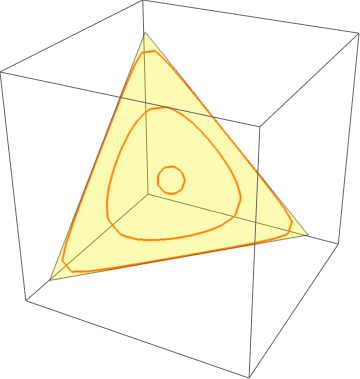
\includegraphics[scale=0.3]{figures/dos0}
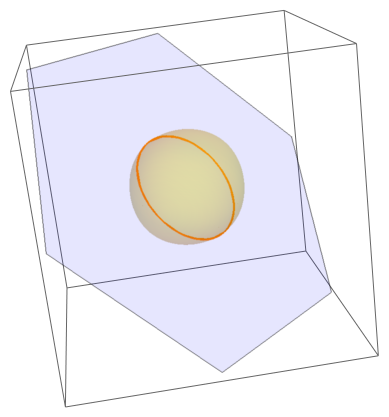
\includegraphics[scale=0.3]{figures/dos1}
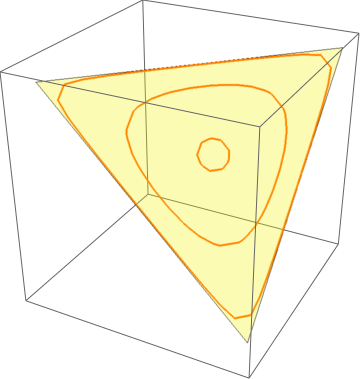
\includegraphics[scale=0.3]{figures/dos2}
\caption{Integration region $\partial\Omega'$ with contour mesh
representing isosurfaces of the integrand}
\label{fig:dos}
\end{figure}
\noindent
In the one dimensional case the delta function filters the integrand
and there are no more integrals left to do so one obtains the density
directly. In the two dimensional case rotating into the plane of the
constraint $\bar{\mathbf{v}}=\mathbf{R}(\frac{\pi}{4})\bar{\mathbf{u}}$
--- where $\mathbf{R}(\theta)$ is the rotation matrix --- simplifies
the limits and reveals yet another symmetry $\Lambda\rightarrow-\Lambda$.
The final integral yields a complete elliptic integral of the first kind $K(m)$.
\begin{align*}
  \iint_{-2}^{2}\!
  \frac{\delta(\Lambda_2+u+u')}
  {\sqrt{(1-\frac{1}{4}u^2)(1-\frac{1}{4}u'^2)}}
  \,\mathrm{d}u\mathrm{d}u'
  &=
  \iint_{-2}^{2}\!
  \frac{\delta(\Lambda_2+v\sqrt{2})}
  {\sqrt{(1-\frac{1}{8}(v+v')^2)(1-\frac{1}{8}(v-v')^2)}}
  \,\mathrm{d}v\mathrm{d}v'\\
  &=
  \int_{-2\sqrt{2}+\frac{\sqrt{2}}{2}|\Lambda_2|}^{2\sqrt{2}-\frac{\sqrt{2}}{2}|\Lambda_2|}\!
  \frac{1}
  {\sqrt{(1-\frac{1}{8}(v'+\frac{\Lambda_2}{\sqrt{2}})^2)(1-\frac{1}{8}(v'-\frac{\Lambda_2}{\sqrt{2}})^2)}}
  \,\mathrm{d}v'\\
  &\sim
  \frac{1}{|\Lambda_2|+4}
  K\left(\left(\frac{|\Lambda_2|-4}{|\Lambda_2|+4}\right)^2\right)
\end{align*}
\begin{align}
  \therefore \rho_1(\lambda)=
  \frac{1}
  {2\pi\sqrt{1-\frac{1}{4}(\lambda+2)^2}}
  \qquad
  \rho_2(\lambda)=\frac{4\pi^{-2}}{|\lambda+4|+4}
    K\left(\left(\frac{|\lambda+4|-4}{|\lambda+4|+4}\right)^2\right)
\end{align}
\end{document}
